\let\negmedspace\undefined
\let\negthickspace\undefined
\documentclass[journal]{IEEEtran}
\usepackage[a5paper, margin=10mm, onecolumn]{geometry}
%\usepackage{lmodern} % Ensure lmodern is loaded for pdflatex
\usepackage{tfrupee} % Include tfrupee package

\setlength{\headheight}{1cm} % Set the height of the header box
\setlength{\headsep}{0mm}     % Set the distance between the header box and the top of the text

\usepackage{gvv-book}
\usepackage{gvv}
\usepackage{cite}
\usepackage{amsmath,amssymb,amsfonts,amsthm}
\usepackage{algorithmic}
\usepackage{graphicx}
\usepackage{textcomp}
\usepackage{xcolor}
\usepackage{txfonts}
\usepackage{listings}
\usepackage{enumitem}
\usepackage{mathtools}
\usepackage{gensymb}
\usepackage{comment}
\usepackage[breaklinks=true]{hyperref}
\usepackage{tkz-euclide} 
\usepackage{listings}
% \usepackage{gvv}                                        
\def\inputGnumericTable{}                                 
\usepackage[latin1]{inputenc}                                
\usepackage{color}                                            
\usepackage{array}                                            
\usepackage{longtable}                                       
\usepackage{calc}                                             
\usepackage{multirow}                                         
\usepackage{hhline}                                           
\usepackage{ifthen}                                           
\usepackage{lscape}
\usepackage{circuitikz}
\tikzstyle{block} = [rectangle, draw, fill=blue!20, 
    text width=4em, text centered, rounded corners, minimum height=3em]
\tikzstyle{sum} = [draw, fill=blue!10, circle, minimum size=1cm, node distance=1.5cm]
\tikzstyle{input} = [coordinate]
\tikzstyle{output} = [coordinate]
\begin{document}

\bibliographystyle{IEEEtran}
\vspace{3cm}

\title{1.11.9}
\author{AI25BTECH11007}
 \maketitle
% \newpage
% \bigskip
{\let\newpage\relax\maketitle}

\renewcommand{\thefigure}{\theenumi}
\renewcommand{\thetable}{\theenumi}
\setlength{\intextsep}{10pt} % Space between text and floats


\numberwithin{equation}{enumi}
\numberwithin{figure}{enumi}
\renewcommand{\thetable}{\theenumi}
\noindent
\textbf{Question:}\\
If
\[
\vec{a} = \hat{i} - 7\hat{j} + 7\hat{k}
\quad \text{and} \quad
\vec{b} = 3\hat{i} - 2\hat{j} + 2\hat{k},
\]
find a unit vector perpendicular to both the vectors $\vec{a}$ and $\vec{b}$.\\
\textbf{Solution:}\\
A vector perpendicular to both $\vec{a}$ and $\vec{b}$ is given by
\[
\vec{n} = \vec{a} \times \vec{b}.
\]

\[
\vec{n} =
\begin{vmatrix}
\hat{i} & \hat{j} & \hat{k} \\
1 & -7 & 7 \\
3 & -2 & 2
\end{vmatrix}.
\]

Expanding,
\[
\vec{n} = \myvec{0 \\ 19 \\ 19}.
\]

The magnitude is
\[
|\vec{n}| = \sqrt{0^2 + 19^2 + 19^2} = 19\sqrt{2}.
\]

Hence the required unit vector is
\[
\hat{n} = \frac{\vec{n}}{|\vec{n}|}
= \frac{1}{19\sqrt{2}} \myvec{0 \\ 19 \\ 19}
= \myvec{0 \\ \tfrac{1}{\sqrt{2}} \\ \tfrac{1}{\sqrt{2}}}.
\]

Therefore, a unit vector perpendicular to both $\vec{a}$ and $\vec{b}$ is
\[
\hat{n} = \frac{1}{\sqrt{2}}(\hat{j} + \hat{k}),
\]
or its negative.

\begin{figure}[H]
    \centering
    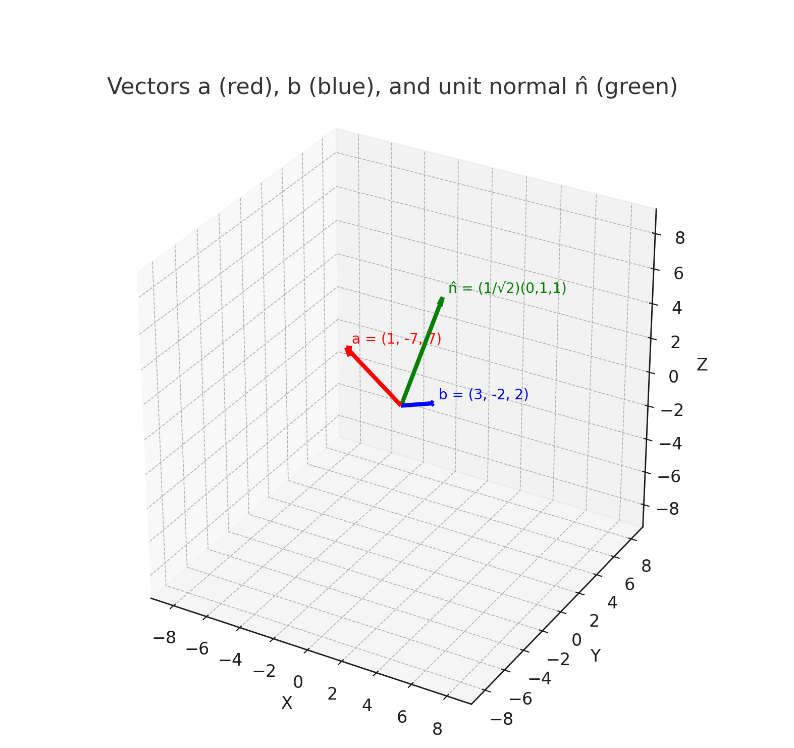
\includegraphics[width=0.75\columnwidth]{figs/image.png}
    \caption{Image Visual}
    \label{fig:figs/image.png}
\end{figure}
  
\end{document}
